\newpage
\begin{Pro}
   Convierte las siguientes expresiones regulares en autómatas finitos deterministas (DFA):
   \begin{enumerate}
       \item $[ab]^*$
       \item $(a?b^*)^*$
       \item $[ab]^*abb[ab]^*$
    \end{enumerate}
\end{Pro}

\begin{enumerate}
    \item $[ab]^*$
    Primero aplicamos el algoritmo de Thompson para construir el AFN:
    \begin{figure}[h!]
        \centering
        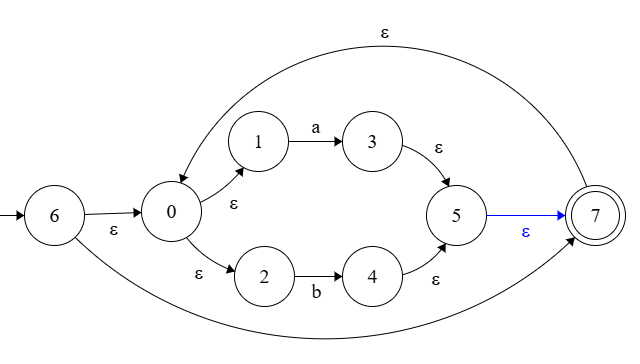
\includegraphics[width=0.5\textwidth]{images/7a.png}
        \caption{Automata Finito No Determinista, ejercicio 7 a}
    \end{figure}\\
    donde el estado inicial es $6$ y el estado final es $7$.

    Ahora convertimos el AFN en un AFD:
    Primero vamos a sacar las epsilon cerradura de cada estado:
    \begin{itemize}
        \item $\epsilon$-Cerradura($6$) = $\{0,1,2,6,7\}$
        \item $\epsilon$-Cerradura($1$) = $\{1\}$
        \item $\epsilon$-Cerradura($2$) = $\{2\}$
        \item $\epsilon$-Cerradura($3$) = $\{0,1,2,3,5,7\}$
        \item $\epsilon$-Cerradura($4$) = $\{0,1,2,4,5,7\}$
        \item $\epsilon$-Cerradura($5$) = $\{0,1, 2, 5, 7\}$
        \item $\epsilon$-Cerradura($7$) = $\{0,1,2, 7\}$
    \end{itemize}
    \newpage
    Ahora vamos a construir la tabla de transiciones del AFD:\\
    \begin{table}[h!]        
    \centering
    \begin{tabular}{|c|c|c|}
    \hline
    \textbf{Estados} & \textbf{Transición con a} & \textbf{Transición con b } \\
    \hline
    $\epsilon$-Cerradura($6$) &$\epsilon$-Cerradura($3$) & $\epsilon$-Cerradura($4$)\\
    \hline      
    $\epsilon$-Cerradura($3$) & $\epsilon$-Cerradura($3$) & $\epsilon$-Cerradura($4$) \\
    \hline 
    $\epsilon$-Cerradura($4$) & $\epsilon$-Cerradura($3$) & $\epsilon$-Cerradura($4$) \\
    \hline
    \end{tabular}
    \caption{Tabla de transiciones del AFD} 
    \end{table}\\
    Entonces el AFD queda así:\\
    \begin{figure}[h!]
        \centering
        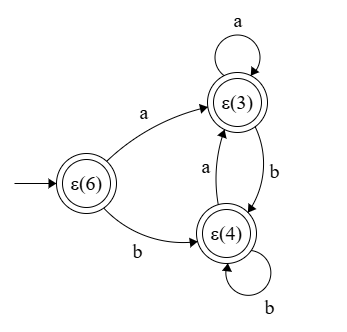
\includegraphics[width=0.5\textwidth]{images/7aDFA.png}
        \caption{Automata Finito Determinista, ejercicio 7 a}
    \end{figure}\\
    Si lo minimizamos, queda así:

    \begin{figure}[!ht]  
        \centering
        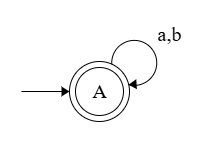
\includegraphics[width=0.5\textwidth]{images/7bDFAminimo.png}
        \caption{Automata Finito Determinista Mínimo, ejercicio 7 a}
    \end{figure}

    \newpage
    \item $(a?b^*)^*$
    Vamos a construir primero el AFN, con el algoritmo de Thompson:
    
    \begin{figure}[h!]
        \centering
        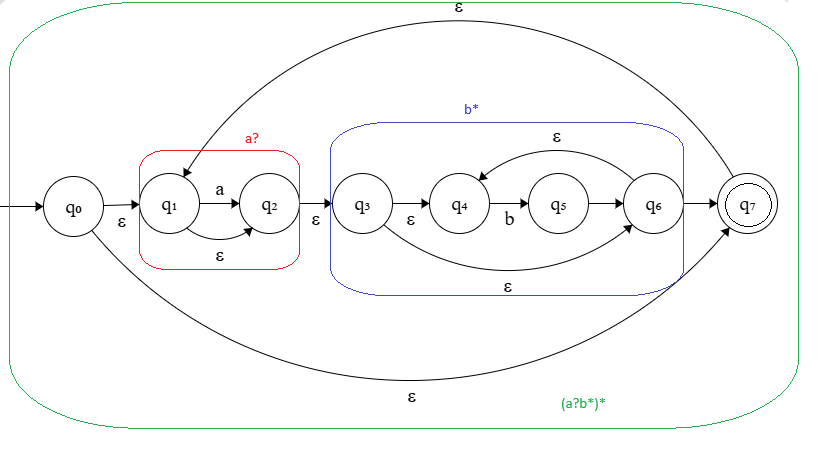
\includegraphics[width=0.5\textwidth]{images/7bAFN.png}
        \caption{Automata Finito No Determinista, ejercicio 7 b}
    \end{figure}

    Ahora vamos a convertir el AFN en un AFD, con el algoritmo de subconjuntos:
    Primero vamos a sacar las epsilon cerradura de cada estado:
    \begin{itemize}
        \item $\epsilon$-Cerradura($q_0$) = $\{q_0, q_1, q_2, q_3, q_4, q_6, q_7\}$
        \item $\epsilon$-Cerradura($q_1$) = $\{q_1, q_2, q_3, q_4, q_6, q_7\}$
        \item $\epsilon$-Cerradura($q_2$) = $\{q_1, q_2, q_3, q_4, q_6, q_7\}$
        \item $\epsilon$-Cerradura($q_3$) = $\{q_1, q_2, q_3, q_4, q_6, q_7\}$
        \item $\epsilon$-Cerradura($q_4$) = $\{q_4\}$
        \item $\epsilon$-Cerradura($q_5$) = $\{q_1, q_2, q_3, q_4, q_5, q_6, q_7\}$
        \item $\epsilon$-Cerradura($q_6$) = $\{q_1, q_2, q_3, q_4, q_6, q_7\}$
        \item $\epsilon$-Cerradura($q_7$) = $\{q_1, q_2, q_3, q_4, q_6, q_7\}$
    \end{itemize}
    Ahora vamos a construir la tabla de transiciones del AFD:
    \begin{table}[h!]        
    \centering
    \begin{tabular}{|c|c|c|}
    \hline
    \textbf{Estados} & \textbf{Transición con a} & \textbf{Transición con b } \\
    \hline
    $\epsilon$-Cerradura($q_0$) &$\epsilon$-Cerradura($q_2$) & $\epsilon$-Cerradura($q_5$) \\
    \hline      
    $\epsilon$-Cerradura($q_2$) & $\epsilon$-Cerradura($q_2$) & $\epsilon$-Cerradura($q_5$) \\
    \hline 
    $\epsilon$-Cerradura($q_5$) & $\epsilon$-Cerradura($q_2$) & $\epsilon$-Cerradura($q_5$)\\
    \hline
    \end{tabular}
    \caption{Tabla de transiciones del AFD} 
    \end{table}

    Vease que el automata queda así: \\

    \begin{figure}[h!]
        \centering
        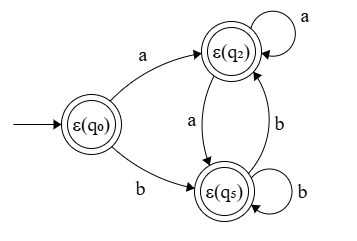
\includegraphics[width=0.5\textwidth]{images/7bDFAnoMinimizado.png}
        \caption{Automata Finito Determinista, ejercicio 7 b}
    \end{figure}
    \newpage

    Sí aplicamos el algoritmo de minimización de DFA, queda de la siguiente manera: \\
    \begin{figure}[h!]
        \centering
        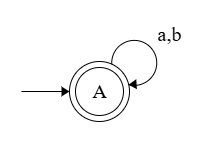
\includegraphics[width=0.5\textwidth]{images/7bDFAminimo.png}
        \caption{Automata Finito Determinista Mínimo, ejercicio 7 b}
    \end{figure}
\newpage
    \item $[ab]^*abb[ab]^*$ \\
    Note que el autómata para $[ab]^*$ es: \\
    \begin{figure}[h!]   
        \centering
        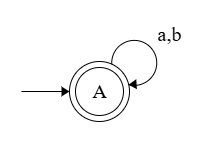
\includegraphics[width=0.5\textwidth]{images/7bDFAminimo.png}
        \caption{Automata Finito Determinista, $[ab]^*$}
    \end{figure} \\
    Ahora vamos a construir el autómata para $[ab]^*abb[ab]^*$: \\
    \begin{figure}[h!]
        \centering
        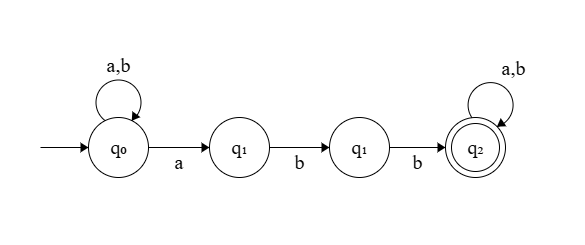
\includegraphics[width=0.5\textwidth]{images/7c.png}
        \caption{Automata Finito Determinista, ejercicio 7 c}
    \end{figure}
\end{enumerate}